\documentclass[12pt, a4paper]{article}
%\usepackage{a4wide}%
\usepackage{geometry}
\usepackage{ucs}
\usepackage{caption}
\usepackage{graphicx}
\usepackage[T1]{fontenc}
\usepackage{selinput} 
\usepackage[german]{babel}
\usepackage{float}
\usepackage{listings}
\usepackage{lastpage}
\usepackage{amsmath}

\inputencoding{latin2}
\inputencoding{utf8}

\geometry{,
  margin=2.54cm
}

\SelectInputMappings{ 
  adieresis={ä}, 
  germandbls={ß}, 
  Euro={€} 
}

\pagenumbering{arabic}
\usepackage{color}
\definecolor{softGray}{RGB}{160,160,160}
\definecolor{softOrange}{RGB}{255,140,15}
\definecolor{darkGreen}{RGB}{35,110,37}
\definecolor{darkRed}{RGB}{136,19,80}
\definecolor{stringColor}{RGB}{118,15,21}
\definecolor{identColor}{RGB}{0,51,105}
\definecolor{typeColor}{RGB}{0,69,176}
\definecolor{keywordColor}{RGB}{0,69,176}
\definecolor{gray}{RGB}{160,160,160}
\definecolor{lightBlue}{RGB}{44,152,242}
\definecolor{commentColor}{RGB}{135,135,135}
\definecolor{stringColor}{RGB}{221,36,0}
\definecolor{identifierColor}{RGB}{63,110,125}
\definecolor{bluekeywords}{rgb}{0.13,0.13,1}
\definecolor{greencomments}{rgb}{0,0.5,0}
\definecolor{bluestrings}{rgb}{0.13,0.5,0.5}

\author{Rotaru Daniel}
\usepackage{fancyhdr}
\pagestyle{fancy}
\cfoot{\thepage\ of \pageref{LastPage} }

\DeclareUnicodeCharacter{FEFF}{ }

\begin{document}
\lstset{language=csh,
				extendedchars=\true,
				inputencoding=utf8,
				breakatwhitespace=false,
        breaklines=true,
        stepnumber=2,
        basicstyle=\ttfamily\scriptsize,
        columns=fullflexible,
        showspaces=false,
        showstringspaces=false,
        keywordstyle=\bf\color{bluekeywords},
        commentstyle=\color{greencomments},
        stringstyle=\color{bluestrings},
        showtabs=false,
        tabsize=2
        }
\section{Ultimate Festival Organizer (UFO)}

\subsection{Datenmodell}

\begin{figure}[h] 	
	\centering
		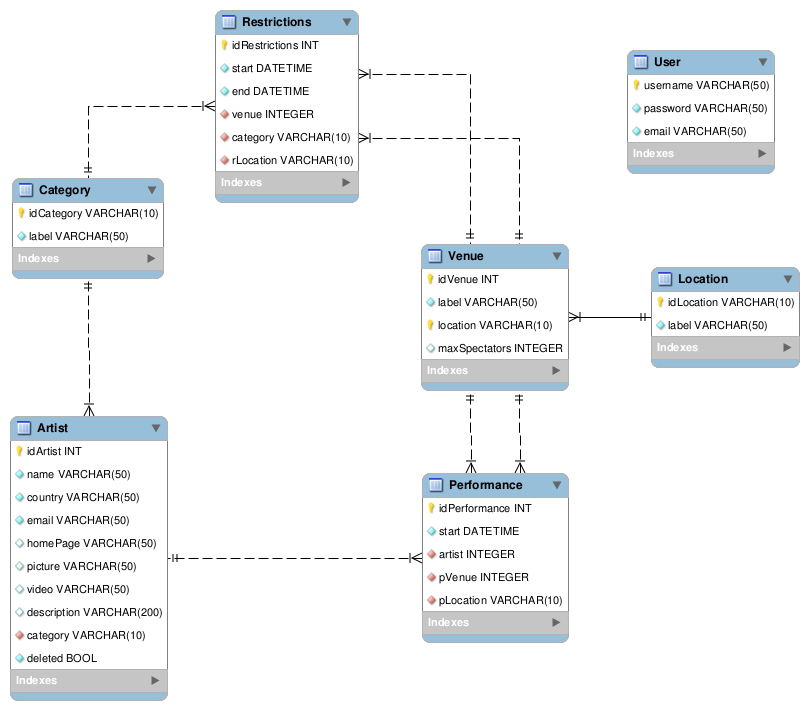
\includegraphics[width=0.7\textwidth]{DbDiagramm.png}
	\caption{OR-Diagramm}
\end{figure}

Das Datenmodell enthält zusätzlich zu den vorgegebenen Entitäten zwei weitere Entitäten: \textit{Location}-Entität und \textit{Restrictions}-Entität. Die \textit{Location}-Entität enthält als Primärschlüssel eine kurze Bezeichnung einer bestimmter Ort und der vollständige Name des Ortes, z.B. H - Hauptplatz, L - Landstraße. Der Primärschlüssel der \textit{Location}-Entität wird als Fremdschlüssel und gleichzeitig Primärschlüssel in der Spielstätte-Entität verwendet. Die Spielstätte-Entität besitzt einen zusammengesetzten Primärschlüssel aus zwei Attributen: \textit{idVenue} und der Fremdschlüssel \textit{location}. Das Attribut \textit{idVenue} wird nicht automatisch inkrementiert, sondern wird von Programm bestimmt, indem man der Anzahl an aktuell existierende Spielstätte für ein bestimmtes Ort um eins inkrementiert und als nächstes \textit{idVenue} speichert. Dadurch schafft man, dass die \textit{idVenue} für ein bestimmtes Ort, z.B. Hauptplatz, nicht größer wird als der Tatsächlichen Anzahl an Spielstätten für diesen Ort.

Die Entität \textit{Restrictions} kann benutzt werden, um bestimmte Darbietungskategorien einschränken zu können. Zum Beispiel kann eine mögliche Kategorie für Kinder so eingeschränkt, dass die Aufführungen für Kinder nur während einer bestimmten Zeitspanne vorgetragen werden können. Auch Feueraufführungen sollen nur zwischen 21 und 23 Uhr stattfinden, da zu diesem Zeitpunkt das Tageslicht nicht mehr so stakt ist. 

Die Entität \textit{Artist} Besitz ein Attribut der Typ Bool \textit{deleted}, der gesetzt wird, falls ein Künstler gelöscht werden soll. Damit wird der Künstler als gelöscht markiert, wird aber nicht aus der Datenbank gelöscht.

\subsection{Datenzugriffsschicht}

Um eine möglich gute Abstraktion zu erreichen, wurde für jede Domainklasse eine \textit{Dao} Interface angelegt. Die Daten aus der Datenbank können nur über die Methoden, die im jeweilige Interface deklariert wurden, zugegriffen werden.

\begin{figure}[h] 	
	\centering
		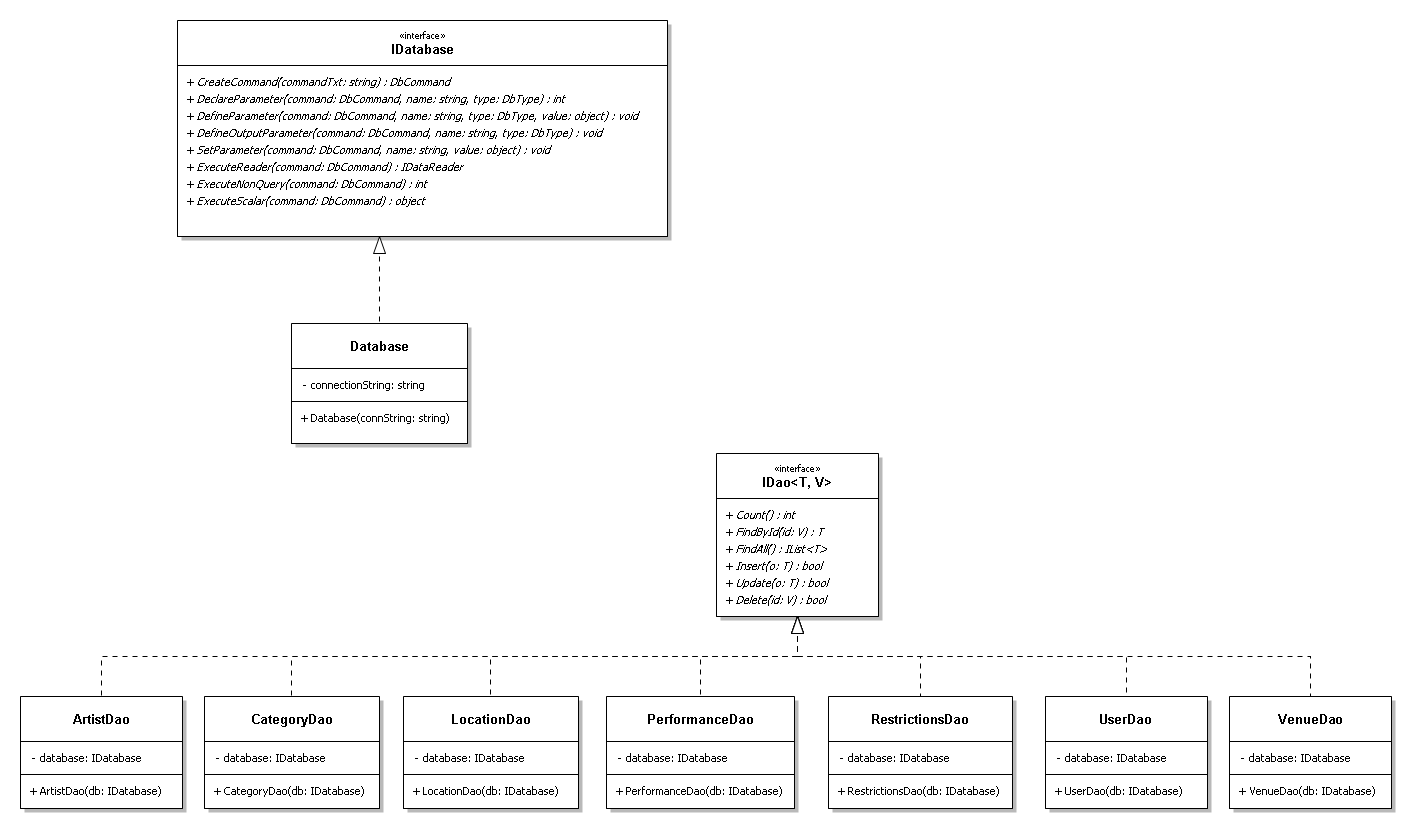
\includegraphics[width=0.7\textwidth]{Dao.png}
	\caption{Data Access}
\end{figure}

Um die Daten besser zwischen unterschiedlichen Schichten zu transportieren, wurde für jede Entität eine eigene \textit{Domain}-Klasse implementiert.

\begin{figure}[h] 	
	\centering
		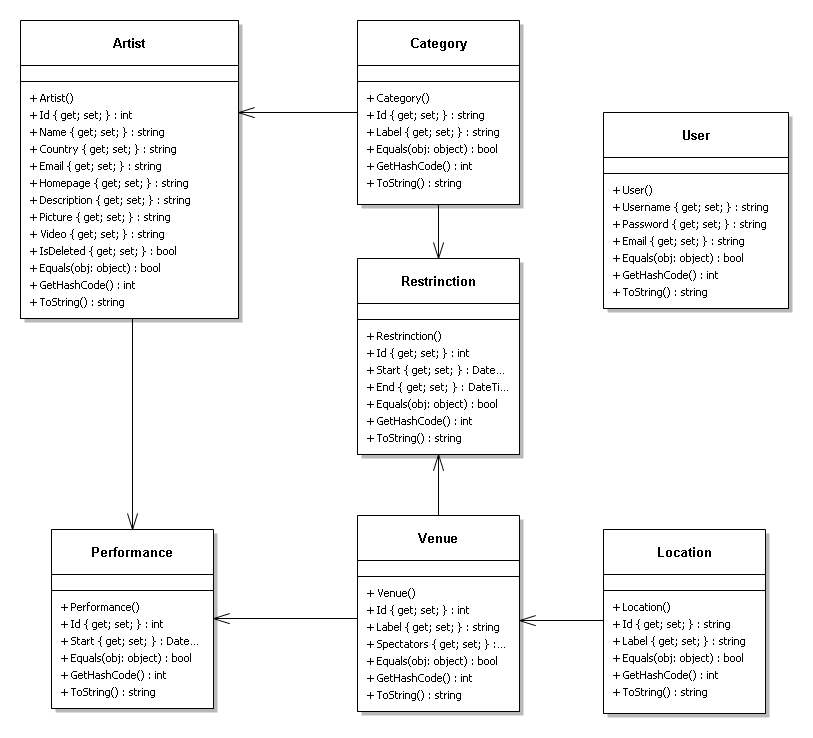
\includegraphics[width=0.6\textwidth]{DomainClasses.png}
	\caption{Domain Classes}
\end{figure}

\clearpage 
\subsubsection{Unit-Tests}

Für jede implementierte DAO-Methode wurde jeweils ein Unit-Test implementiert. Dafür wurde eine eigene Testdatenbank erstellt. Als Testumgebung wurde XUnit-Framework verwendet. Diesen \textit{Framework} bietet ein \textit{AutoRollback}-Attribut, der von Entwickler implementiert werden muss. Diesen Attribut verwendet Datenbanktransaktionen um die Unit-Test Daten nicht in die Datenbank zu speichern. Damit gibt es keine Abhängigkeit zwischen einzelnen Unit-Tests und jeden Unit-Test ist atomar.

\lstinputlisting{../Ufo/Ufo.DAL.Test/AutoRollbackAttribute.cs}

\begin{figure}[h] 	
	\centering
		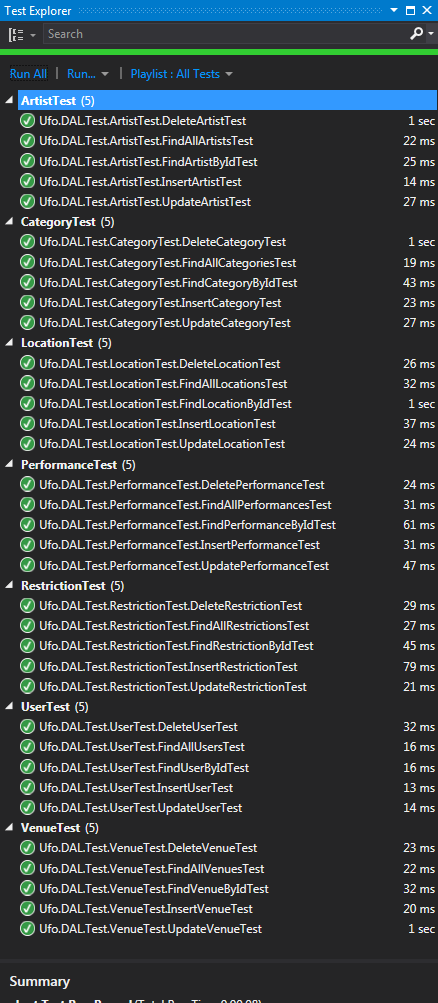
\includegraphics[width=0.5\textwidth]{UnitTests.png}
	\caption{Ergebnis Unit-Tests}
\end{figure}

\clearpage
\subsection{Geschäftslogic}

Die Geschäftslogic ist die einzige Komponente, die mit die Datenzugriffsschicht kommuniziert und stellt die Daten für die Präsentantionsschicht zur Verfügung. Dafür werden zwei Schnittstellen implementiert:

\begin{figure}[h] 	
	\centering
		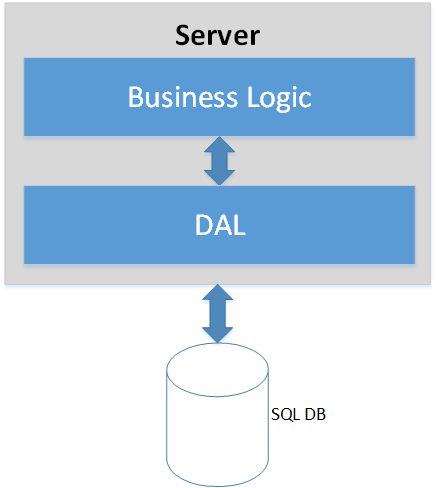
\includegraphics[width=0.5\textwidth]{Server.png}
	\caption{Ergebnis Unit-Tests}
\end{figure}

Die erste Schnittstelle bietet alle Operationen die von UFO Commander verwendet werden. Diese Operationen können verwendet um Benutzer, Kategorien, Künstler, Spielstätten, Aufführungen zu verwalten. 
Es können neue Künstler oder Spielstätte angelegt, neue Kategorien definiert oder Aufführungen von Künstler editieren. Die Präsentationsschicht für den UFO Commander ist nur von diese Schnittstelle abhängig. Die Klasse ManagerImpl implementiert diese Schnittstelle. Um die Geschäftslogic zu verwendet wird eine Factory-Methode zur Verfügung gestellt. Diese Methode erstellt ein Business Logic-Objekt.

Die zweite Schnittstelle stellt alle Informationen zur Verfügung, die auf einem Client angezeigt werden. Das heißt, diese Schnittstelle bietet nur read-only Operationen. Ein Client kann somit nur Daten
anzeigen und keine Daten bearbeiten. Er kann ein Programmübersicht anzeigen oder Informationen von Künstler, Spielstätten und Aufführungen abfragen.Die Klasse ViewerImpl implementiert diese Schnittstelle.

\subsubsection{Unit-Tests}

Für jede Methode aus der Geschäftslogic wurde ein Test-case geschrieben. Damit wird sichergestellt, dass die Geschäftslogic immer die richtige Daten an die höhere Schicht liefert.


\subsection{Präsentationsschicht}

Die Präsentationsschicht für den UFO Commander wird im WPF nach der Model-View-ViewModel Pattern realisiert. Als Model werden die Domainklassen verwendet.

\begin{figure}[h] 	
	\centering
		
\includegraphics[width=0.5\textwidth]{Layers.png}
	\caption{Schichten}
\end{figure}

Der ViewModel wird verwendet, um die Sicht unabhängig von die Domainklassen zu implementieren.

\begin{figure}[h] 	
	\centering
		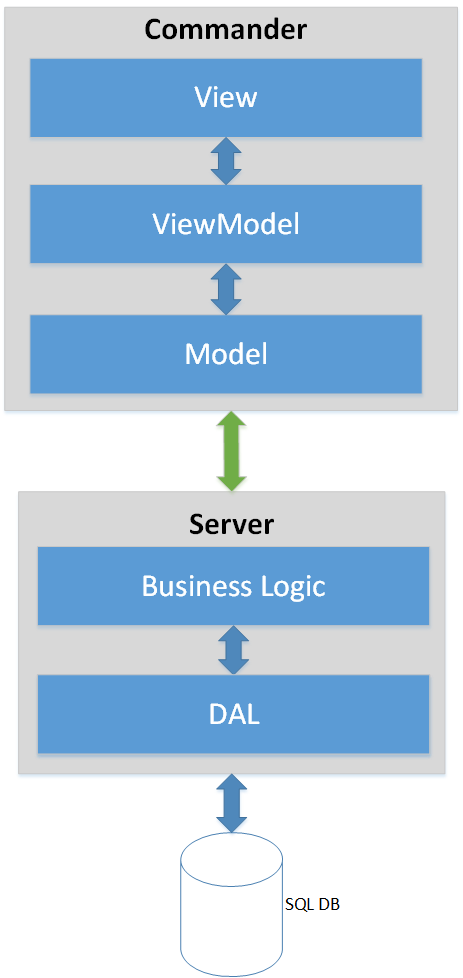
\includegraphics[width=0.4\textwidth]{Arhitecture.png}
	\caption{Komponentenübersicht}
\end{figure}

\subsubsection{Benutzerhandbuch}

Beim starten der Applikation wird der Benutzer aufgefordert, sich mit Benutzername und Kennword anzumelden. Im Datenbank wurde ein Benutzer mit der Name \textit{swk5} und Kennword \textit{swk5} angelegt. Nach der Anmeldung, wird als Startbild der Applikation die Programmübersicht des ersten Tages angezeigt. Hier kann der Benutzer das Programm editieren, indem er eine Kachel anklickt. 


\begin{figure}[h] 	
	\centering
		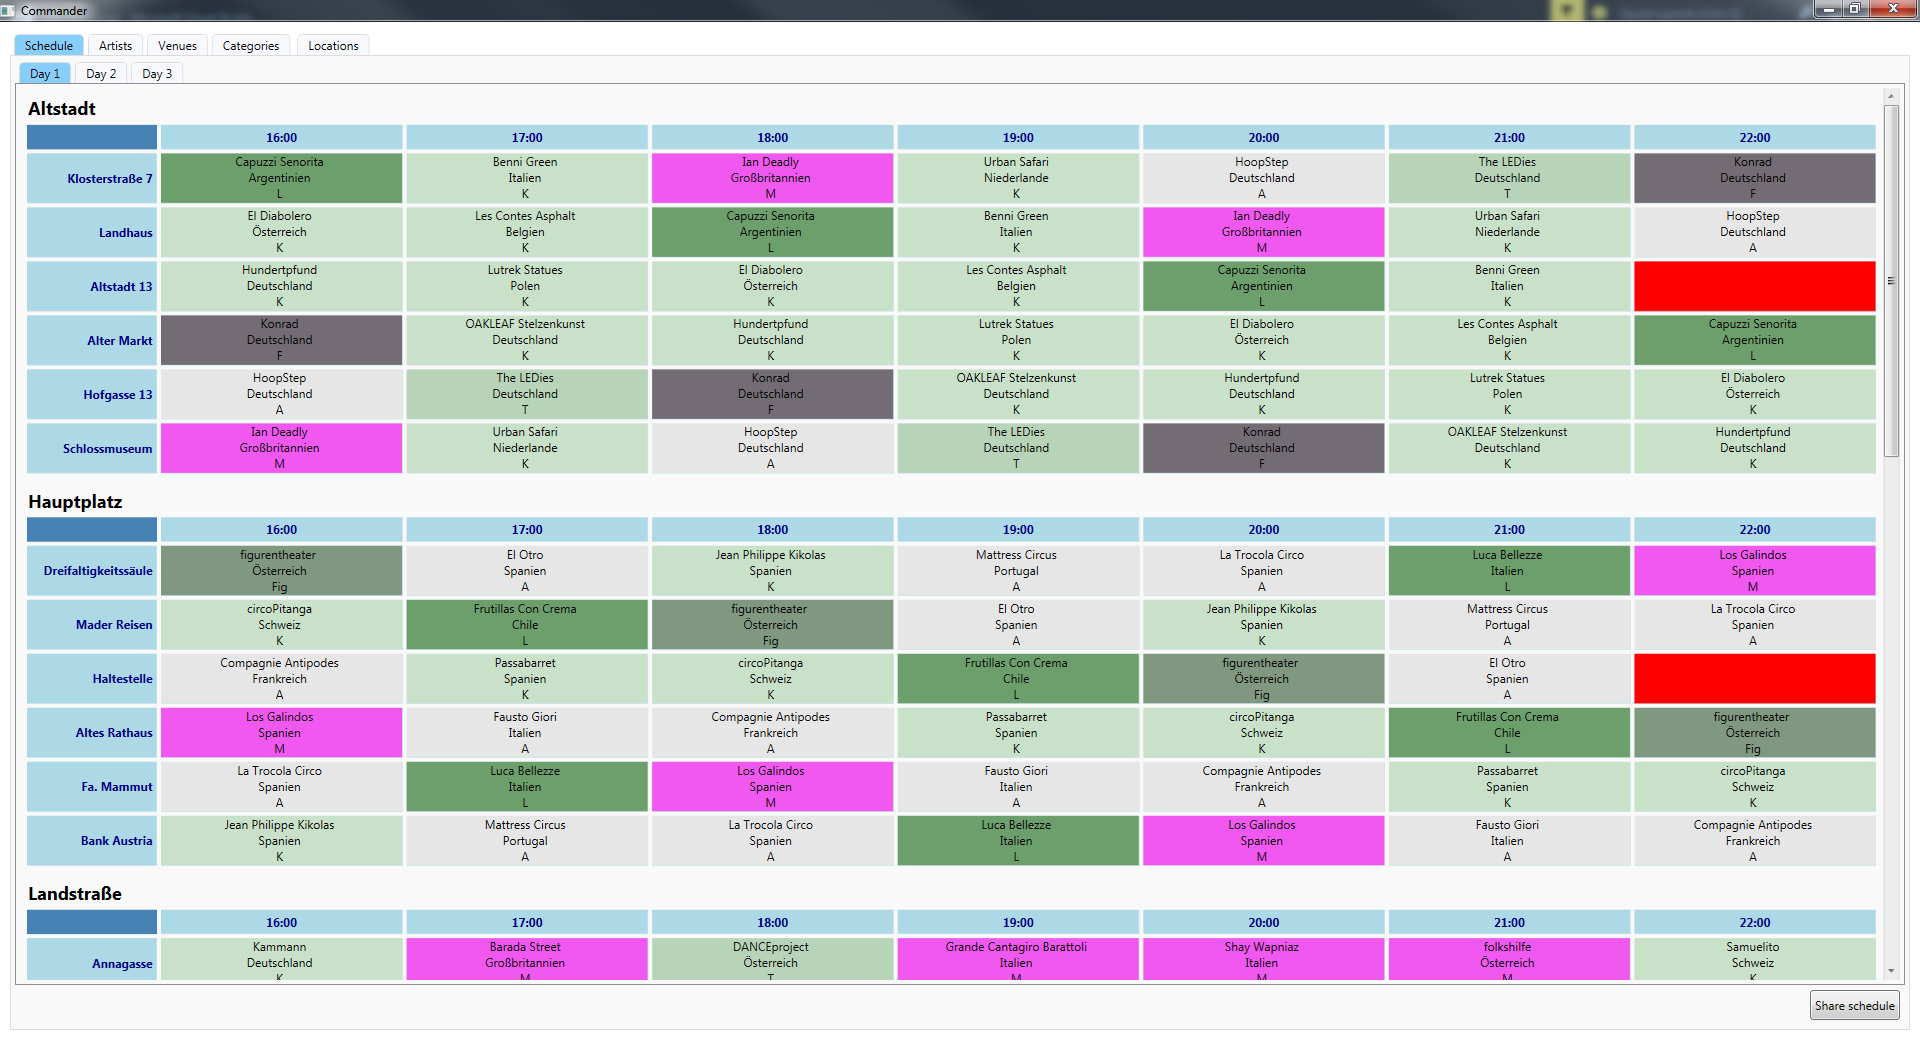
\includegraphics[width=1.0\textwidth]{Startbild.png}
	\caption{Startbild}
\end{figure}

Die Applikation öffnet ein Editierfenster und der Benutzer kann hier aus eine Liste mit alle Künstler ein Künstler auswählen und der Auswahl mit save speichern. Falls der Künstler zu diesem Zeitpunkt, zu keinem anderen Auftritt zugeteilt ist und er zumindest eine Stunden Pause gehabt hat, wird der Künstler gespeichert, ansonsten wird dem Benutzer mitgeteilt, dass diesen Künstler nicht ausgewählt werden kann.

\begin{figure}[h] 	
	\centering
		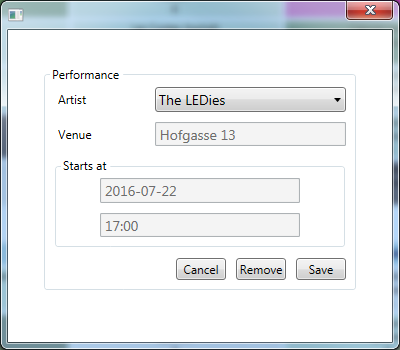
\includegraphics[width=0.5\textwidth]{EditPerformance.png}
	\caption{Aufführung editieren.}
\end{figure}

\clearpage 
Im Reiter \textit{Artists} wird auf die Linke Seite des Fensters eine Liste mit alle im System vorhandene Künstler. Wird ein Künstler ausgewählt, so wird auf die Rechte Seite des Fensters aller Informationen zu dem ausgewählten Künstler angezeigt. Diese Informationen können hier auch editiert und gespeichert werden, oder neue Künstler angelegt.

\begin{figure}[h] 	
	\centering
		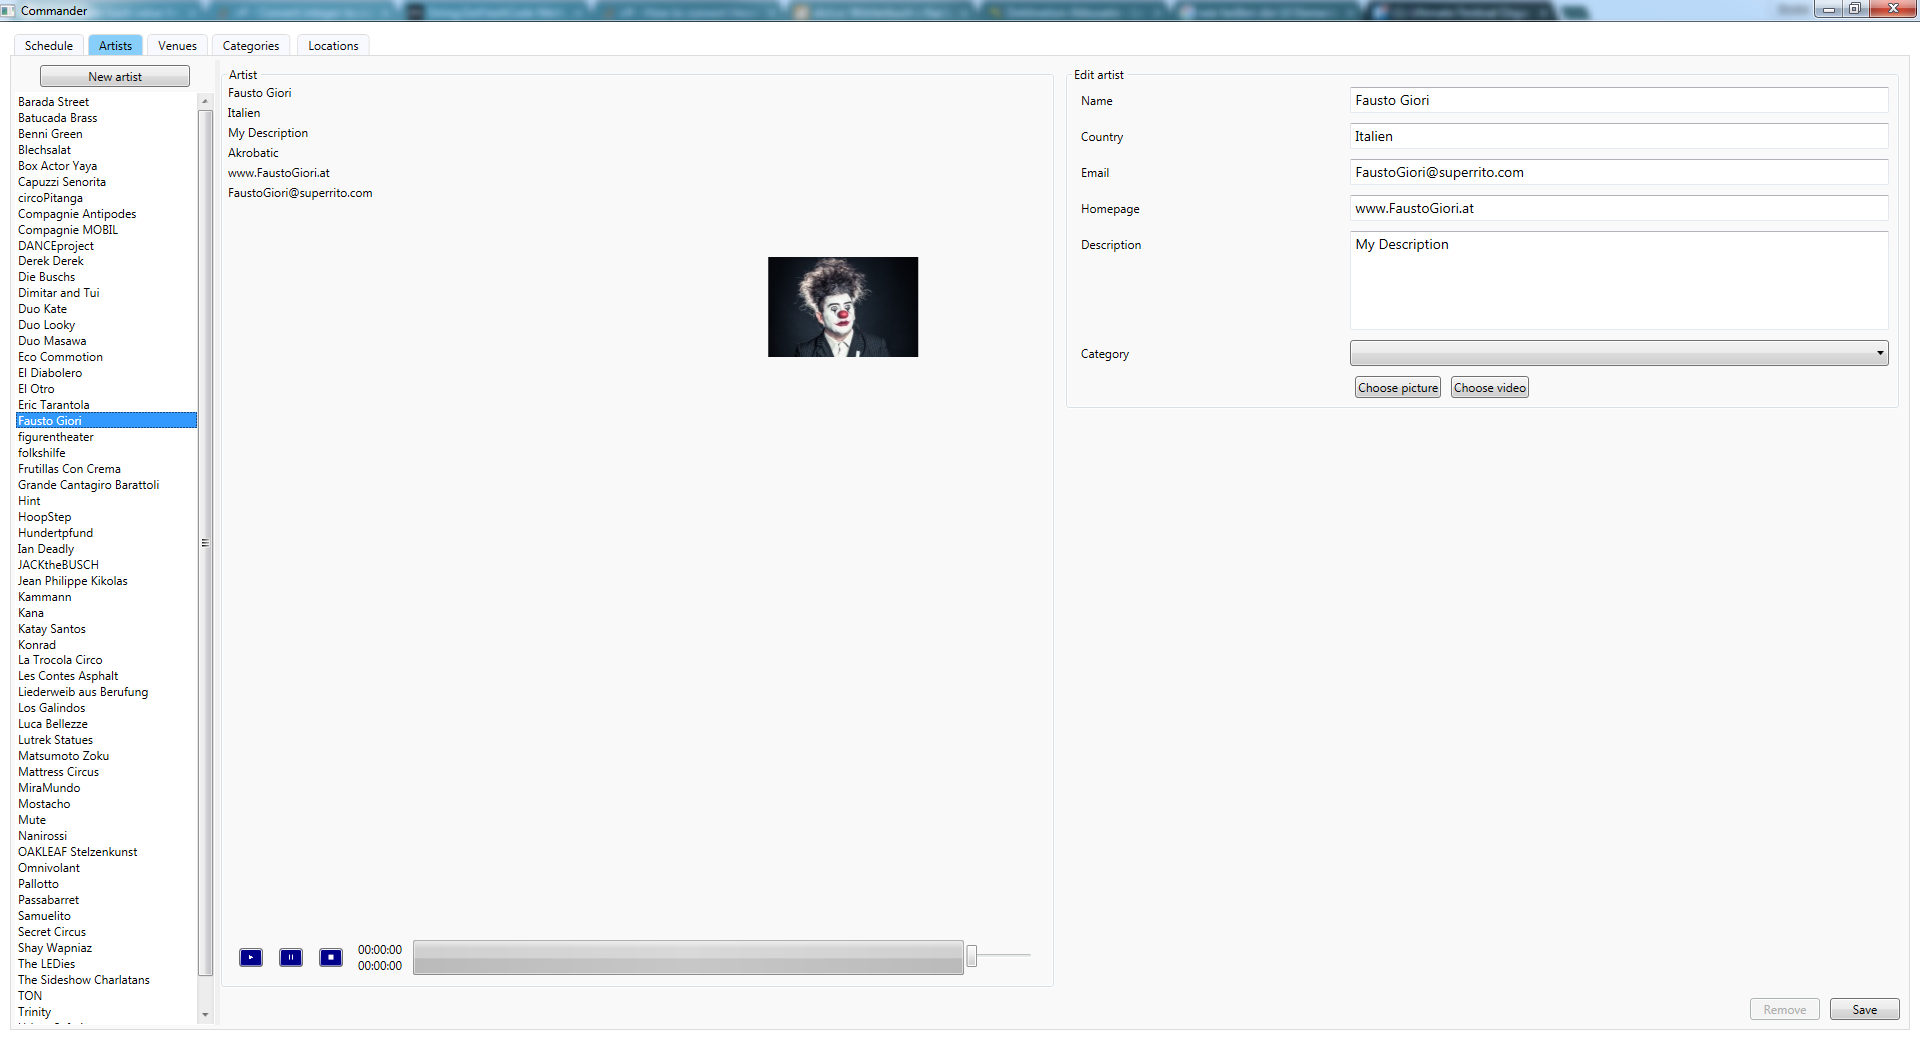
\includegraphics[width=1.0\textwidth]{ArtistWindow.png}
	\caption{Startbild}
\end{figure}
\clearpage 
Im Reiter \textit{Venues} wird auf die Linke Seite des Fensters eine Liste mit alle im System vorhandene Spielstätten. Wird eine Spielstätte ausgewählt, so wird auf die Rechte Seite des Fensters aller Informationen zu der ausgewählte Spielstätte angezeigt. Diese Informationen können hier auch editiert und gespeichert werden, oder neue Spielstätten angelegt.

\begin{figure}[h] 	
	\centering
		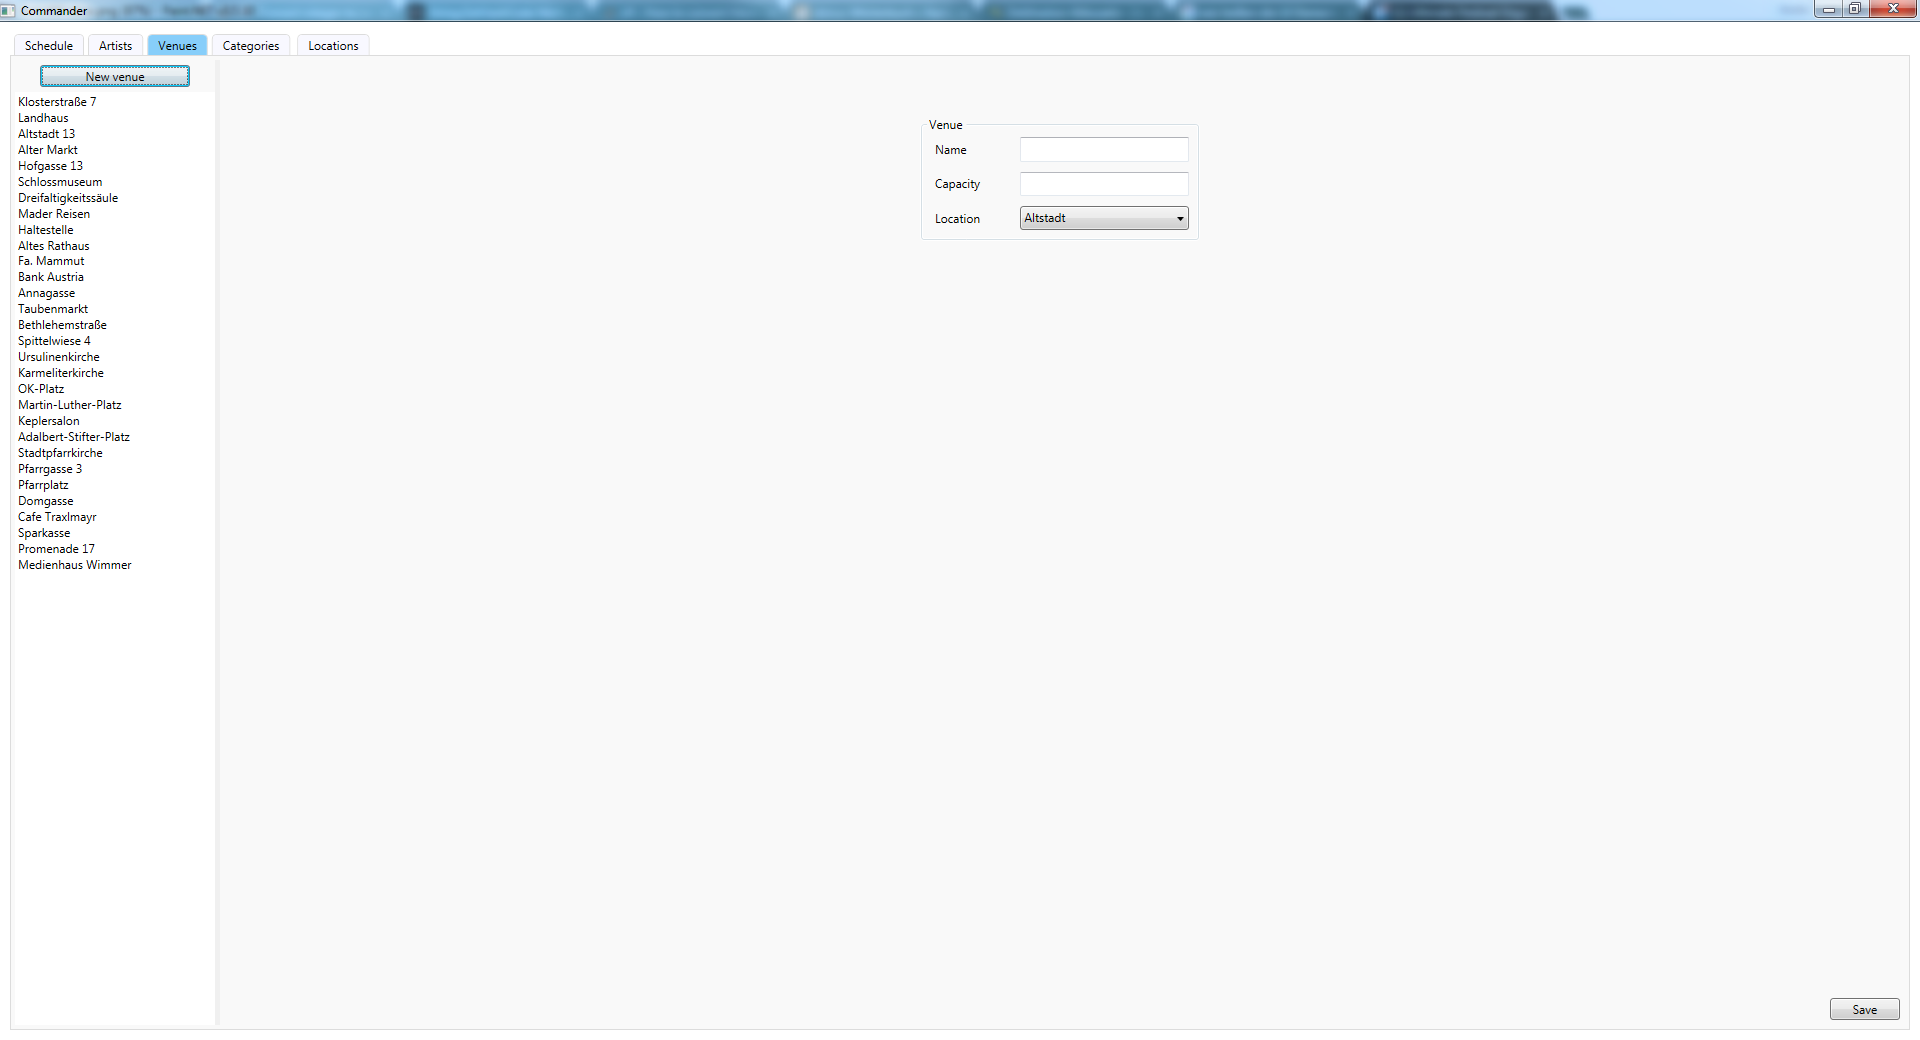
\includegraphics[width=1.0\textwidth]{VenueWindow.png}
	\caption{Startbild}
\end{figure}
\clearpage 
Im Reiter \textit{Categories} wird auf die Linke Seite des Fensters eine Liste mit alle im System vorhandene Kategorien. Wird eine Kategorie ausgewählt, so wird auf die Rechte Seite des Fensters aller Informationen zu der ausgewählte Kategorie angezeigt. Diese Informationen können hier auch editiert und gespeichert werden, oder neue Kategorien angelegt.

\begin{figure}[h] 	
	\centering
		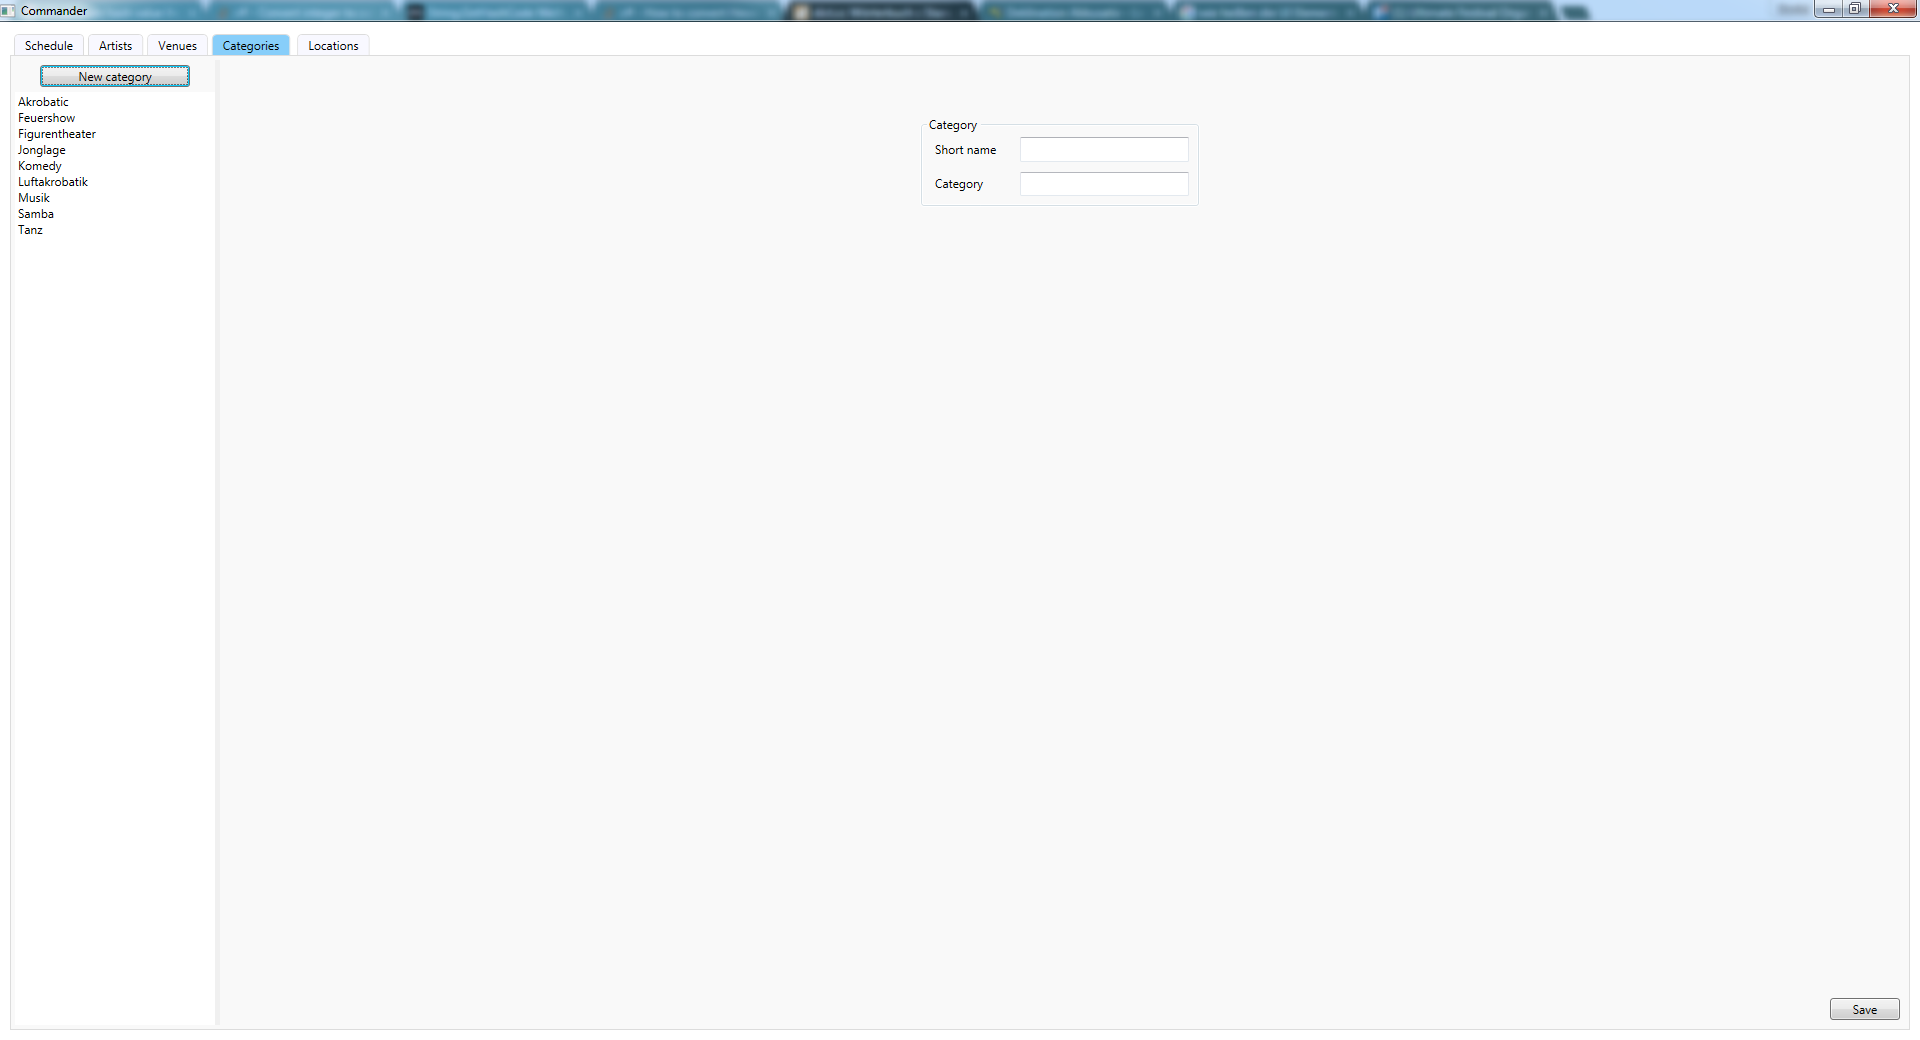
\includegraphics[width=1.0\textwidth]{CategoryWindow.png}
	\caption{Startbild}
\end{figure}
\clearpage 
Im Reiter \textit{Locations} wird auf die Linke Seite des Fensters eine Liste mit alle im System vorhandene Standorte. Wird ein Standort ausgewählt, wird auf die Rechte Seite des Fensters aller Informationen zu dem ausgewählten Standort angezeigt. Diese Informationen können hier auch editiert und gespeichert werden, oder neue Standorte angelegt.

\begin{figure}[h] 	
	\centering
		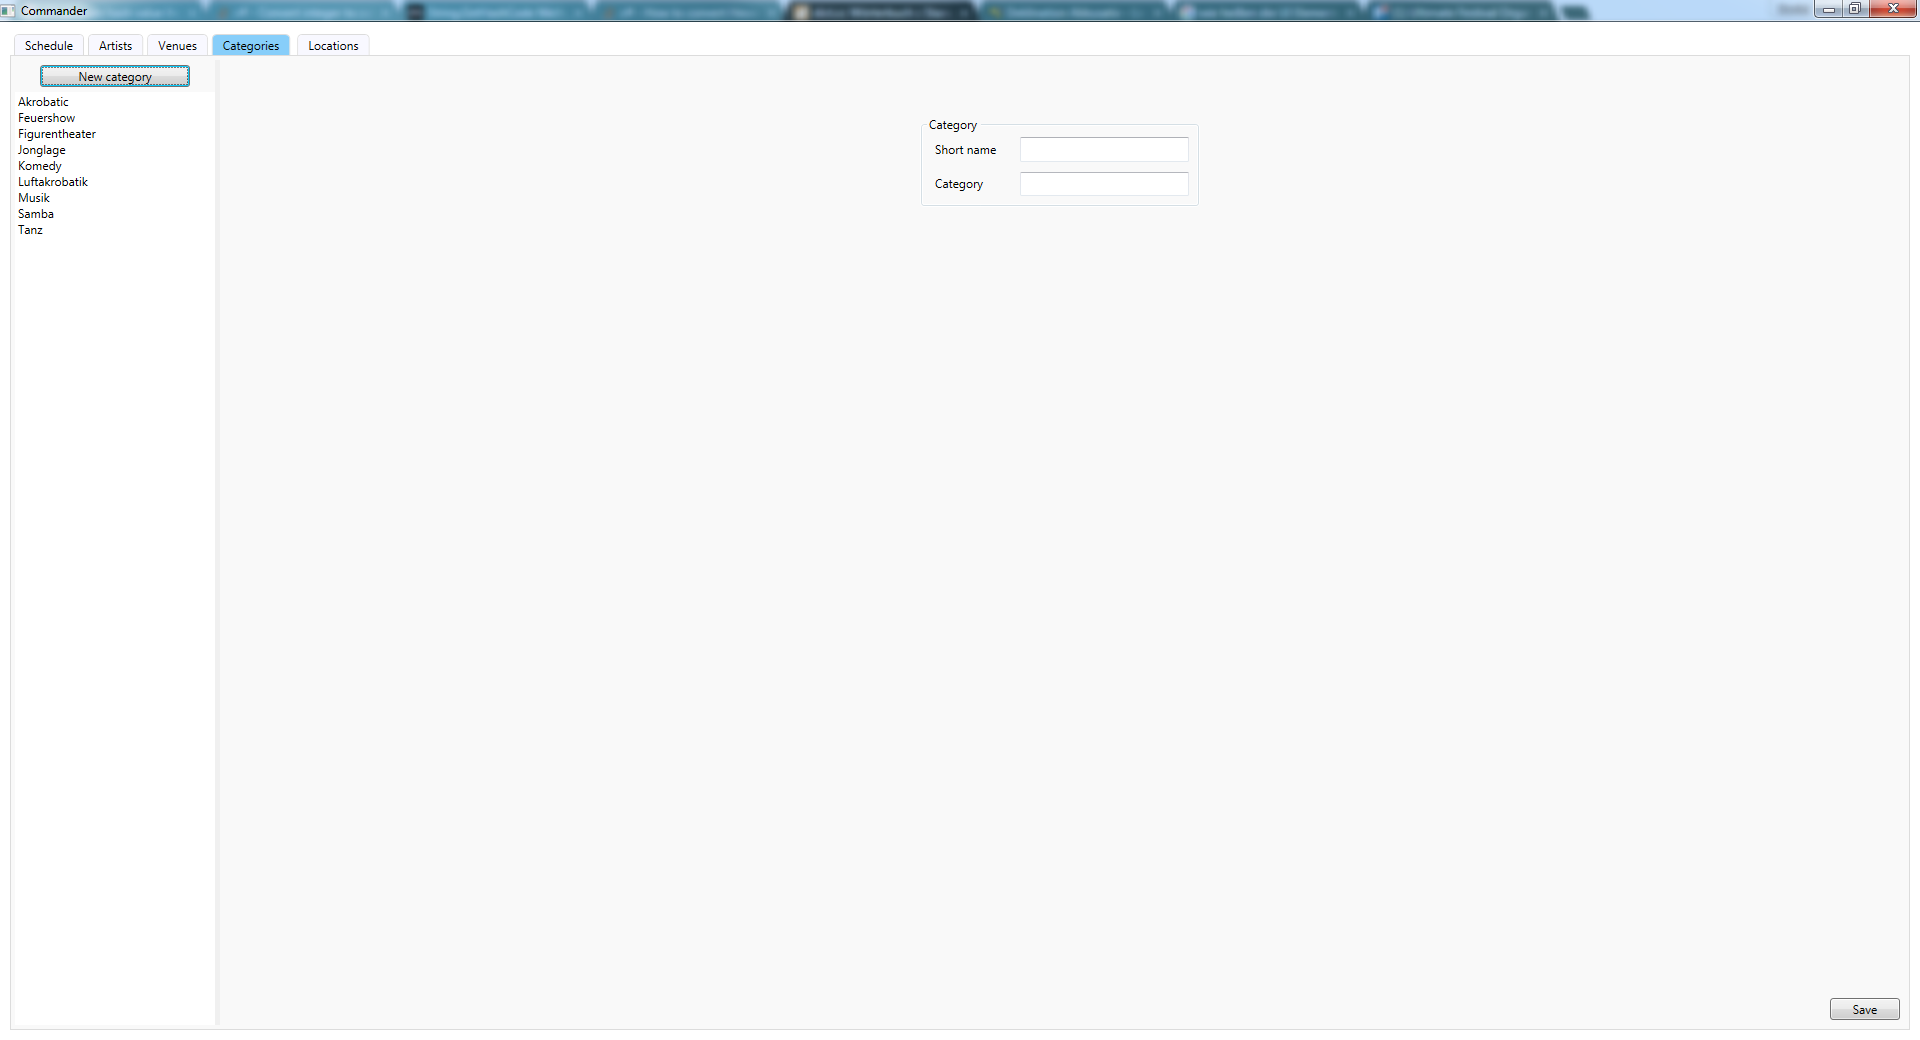
\includegraphics[width=1.0\textwidth]{LocationWindow.png}
	\caption{Startbild}
\end{figure}

\end{document}
